% !TEX TS-program = pdflatex
% !TEX encoding = UTF-8 Unicode

% This is a simple template for a LaTeX document using the "article" class.
% See "book", "report", "letter" for other types of document.

\documentclass[11pt]{article} % use larger type; default would be 10pt

\usepackage[utf8]{inputenc} % set input encoding (not needed with XeLaTeX)

%%% Examples of Article customizations
% These packages are optional, depending whether you want the features they provide.
% See the LaTeX Companion or other references for full information.

%%% PAGE DIMENSIONS
\usepackage{geometry} % to change the page dimensions
\geometry{a4paper} % or letterpaper (US) or a5paper or....
% \geometry{margin=2in} % for example, change the margins to 2 inches all round
% \geometry{landscape} % set up the page for landscape
%   read geometry.pdf for detailed page layout information

\usepackage{graphicx} % support the \includegraphics command and options

% \usepackage[parfill]{parskip} % Activate to begin paragraphs with an empty line rather than an indent

%%% PACKAGES
\usepackage{booktabs} % for much better looking tables
\usepackage{array} % for better arrays (eg matrices) in maths
\usepackage{paralist} % very flexible & customisable lists (eg. enumerate/itemize, etc.)
\usepackage{verbatim} % adds environment for commenting out blocks of text & for better verbatim
\usepackage{subfig} % make it possible to include more than one captioned figure/table in a single float
% These packages are all incorporated in the memoir class to one degree or another...

%%% HEADERS & FOOTERS
\usepackage{fancyhdr} % This should be set AFTER setting up the page geometry
\pagestyle{fancy} % options: empty , plain , fancy
\renewcommand{\headrulewidth}{0pt} % customise the layout...
\lhead{}\chead{}\rhead{}
\lfoot{}\cfoot{\thepage}\rfoot{}

%%% SECTION TITLE APPEARANCE
\usepackage{sectsty}
\allsectionsfont{\sffamily\mdseries\upshape} % (See the fntguide.pdf for font help)
% (This matches ConTeXt defaults)

%%% ToC (table of contents) APPEARANCE
\usepackage[nottoc,notlof,notlot]{tocbibind} % Put the bibliography in the ToC
\usepackage[titles,subfigure]{tocloft} % Alter the style of the Table of Contents
\renewcommand{\cftsecfont}{\rmfamily\mdseries\upshape}
\renewcommand{\cftsecpagefont}{\rmfamily\mdseries\upshape} % No bold!

%%% END Article customizations

%%% The "real" document content comes below...

\title{electricityMap data analyst challenge}
\author{Julie Sainmont}
%\date{} % Activate to display a given date or no date (if empty),
         % otherwise the current date is printed 

\begin{document}
\maketitle

\section{Two electricity zones in Denmark}

Denmark has two electricity zones:
\begin{itemize}
\item The Eastearn part of Denmark covering Zealand with islands and Bornholm is connected to the synchronous electrical grid of Norway, Sweden and Finland. The hydroelectricity produced by Sweeden and Norway provides a stable source of renewable energy that complement the domestique green production of wind energy.
\item The Western part of Denmark is part of the synchronous grid of Continental Europe which is the largest  synchronous electrical grid in the world and includes most of the europeen union
\end{itemize}

\section{Changes of the carbon footprint of electricity throughout the day}
\begin{figure}
  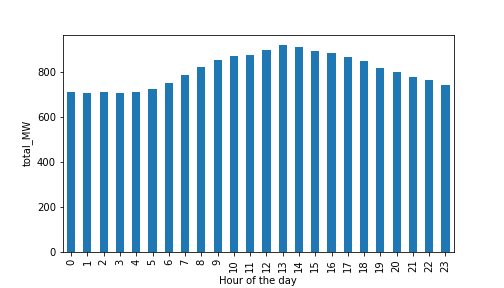
\includegraphics[width=0.8\linewidth]{../outputs/total_MW.png}
  \caption{Energy produced (MWh) throughout the day on average over the year 2020.}
  \label{fig:total_kwh}
\end{figure}
The total energy production varies throughout the day, and is the higher during the day, picking at 1pm (figure \ref{fig:total_kwh}). The demand on the grid for electricity is therefore higher during the day than at night. However to know when it is the best time to use energy, we should looking into the energy sources and their variation accross the day.\\

The energy produced in eastern denmark comes from both renewable sources such as biomass, solar and wind; and from large carbon emitters sources such as gas, oil and coal that come in completement when the energy consumption exceed the production of renewables.\\
When looking at the carbon emission produced per energy (figure \ref{fig:co2_kwh}), we can see that the lowest time is during business hours (8am to 5pm), in particular around 1pm. \\

\begin{figure}
  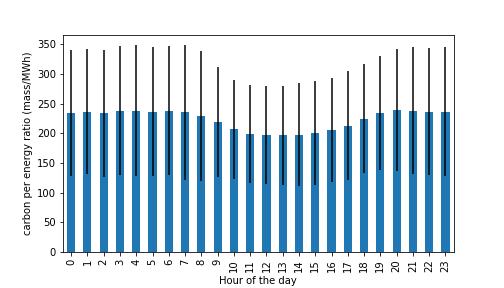
\includegraphics[width=0.8\linewidth]{../outputs/carbon_per_energy_ratio.png}
  \caption{Carbon emitted per energy produced throughout the day on average over the year 2020.}
  \label{fig:co2_kwh}
\end{figure}
 
Similarly if we look at the average fraction of energy produced throughout the day from renewable version non-renewable (figure \ref{fig:per_green}), we can see a similar pattern where the highest renewable energy is produced during the day. 

\begin{figure}
  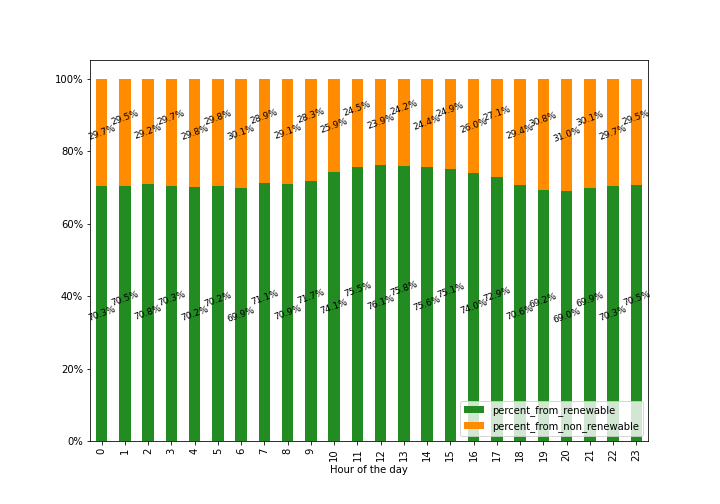
\includegraphics[width=1\linewidth]{../outputs/generated_energy_green_percent.png}
  \caption{Production of renewable and non-renewable energy produced throughout the day on average over the year 2020.}
  \label{fig:per_green}
\end{figure}

\begin{figure}
  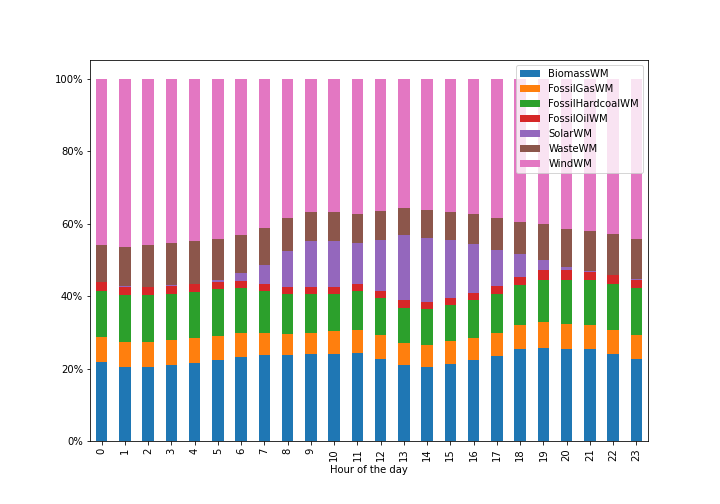
\includegraphics[width=0.9\linewidth]{../outputs/generated_energy_precent_per_sources.png}
  \caption{Production of renewable and non-renewable energy produced throughout the day on average over the year 2020.}
  \label{fig:per_source}
\end{figure}

The renewable energy produced from wind and solar sources are intermittent, however the main diurne variation can be explained by the solar energy production (figure \ref{fig:per_source}, and appendix \ref{app:renewable}, figure \ref{fig:solar_kwh} for a focus on solar production)





\section{Utilizing the data to charge at the greenest time}
In the previous section, we show the average daily variation of the impact of energy on the carbon emission, and showed that on average throughout the day, it is better to use energy during business hours. 
\begin{figure}
  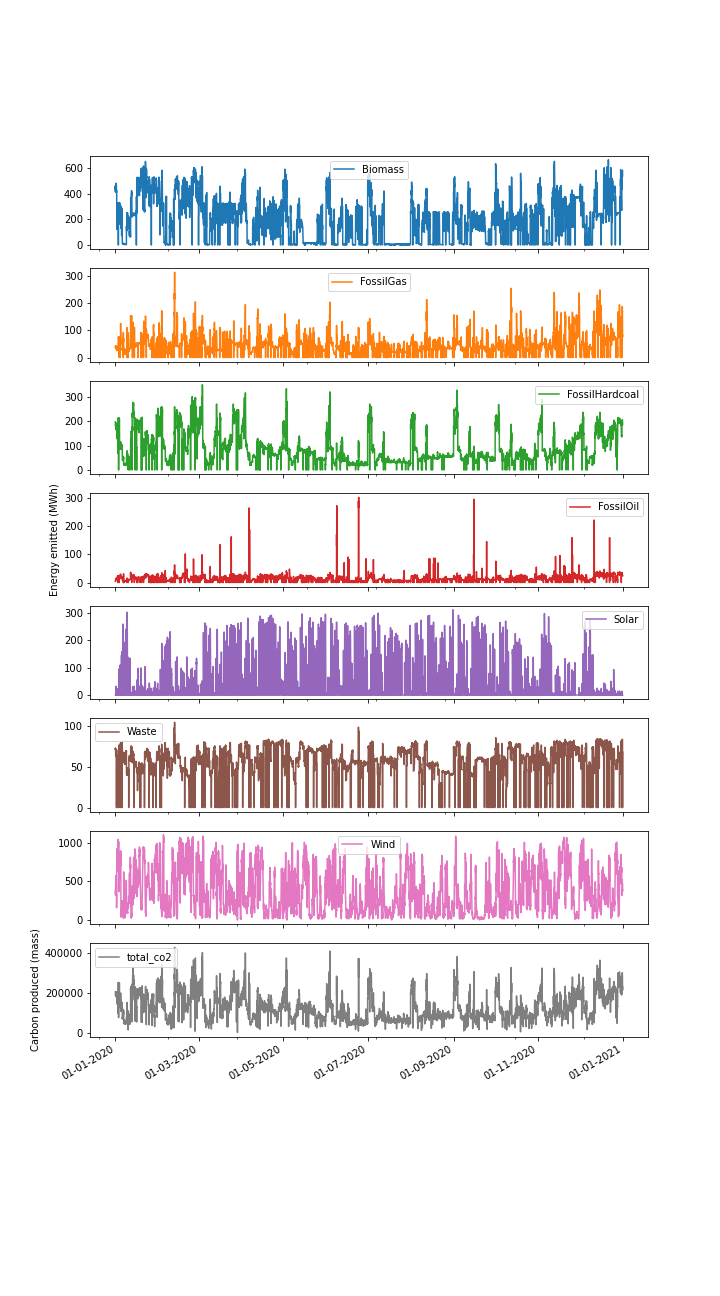
\includegraphics[width=0.7\linewidth]{../outputs/energy_production_time_serie.png}
  \caption{Time serie visualisation of the energy produced in eastern denmark and the carbon emission over the year 2020. The top 6 graphs shows the energy produced from the different sources, and is expressed in kWh, while the bottom graph shows the carbon emission and is expressed in gram of CO$_2$}
  \label{fig:time_series}
\end{figure}



%---  Appendix
\clearpage\newpage
\appendix

\section{Renewable averable production over the day}\label{app:renewable}
% Solar
\begin{figure}[h!]
  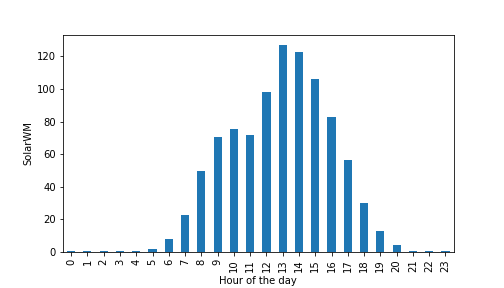
\includegraphics[width=0.8\linewidth]{../outputs/SolarWM.png}
  \caption{Solar energy produced throughout the day in average over the year 2020.}
  \label{fig:solar_kwh}
\end{figure}
% Biomass
\begin{figure}[h!]
  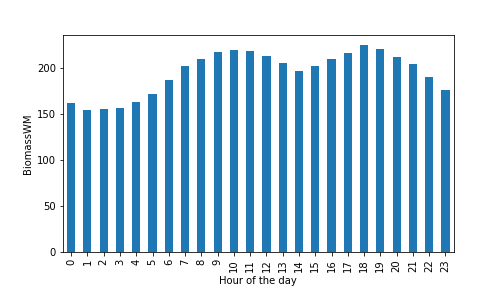
\includegraphics[width=0.8\linewidth]{../outputs/BiomassWM.png}
  \caption{Biomass energy produced throughout the day in average over the year 2020.}
  \label{fig:biomass_kwh}
\end{figure}
% Wind
\begin{figure}[h!]
  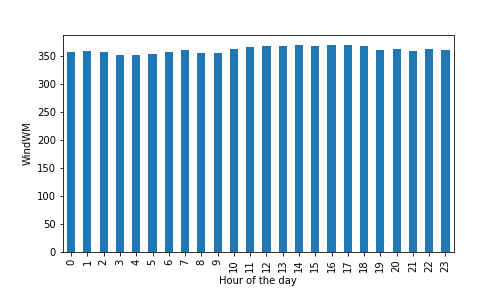
\includegraphics[width=0.8\linewidth]{../outputs/WindWM.png}
  \caption{Wind energy produced throughout the day in average over the year 2020.}
  \label{fig:wind_kwh}
\end{figure}


\clearpage\newpage
\section{Non-renewable averable production over the day}\label{app:non_renewable}
% Gas
\begin{figure}[h!]
  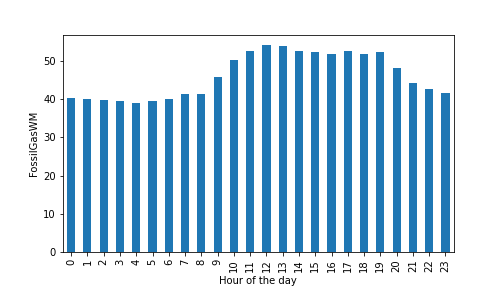
\includegraphics[width=0.8\linewidth]{../outputs/FossilGasWM.png}
  \caption{Fossil gas energy produced throughout the day in average over the year 2020.}
  \label{fig:gas_kwh}
\end{figure}
% coal
\begin{figure}[h!]
  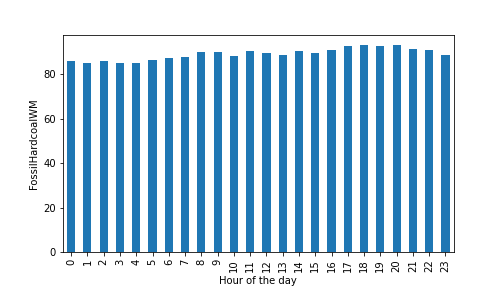
\includegraphics[width=0.8\linewidth]{../outputs/FossilHardcoalWM.png}
  \caption{Fossil hard coal energy produced throughout the day in average over the year 2020.}
  \label{fig:coal_kwh}
\end{figure}
% Oil
\begin{figure}[h!]
  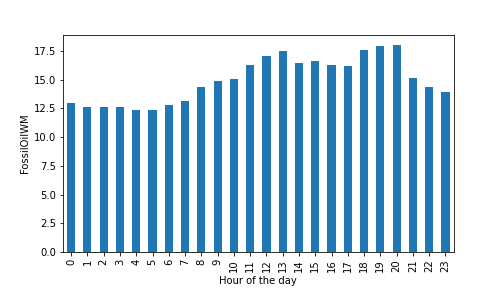
\includegraphics[width=0.8\linewidth]{../outputs/FossilOilWM.png}
  \caption{Fossil Oil energy produced throughout the day in average over the year 2020.}
  \label{fig:oil_kwh}
\end{figure}

\end{document}
